\documentclass[../main/main.tex]{subfiles}

\newdate{date}{20}{11}{2020}


\begin{document}

\marginpar{ \textbf{Lecture 16.} \\  \displaydate{date}. \\ Compiled:  \today.}

\section{Global Invasion Threshold}

Following the formalism introduced for the SIR metapopulation model and markovian mobility, we want now to analytically derive the \textbf{epidemic threshold} for metapopulations. The latter is the \textit{threshold} for a pathogen that, when overcomed, allows it to spread among the entire population. In other words, we want to find the \textbf{conditions} for a \textbf{local outbreak} to \textbf{spread} at a \textbf{global} scale.

\begin{figure}[h!]
\centering
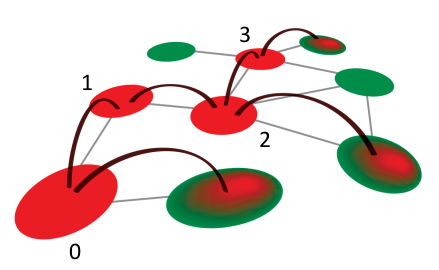
\includegraphics[width=0.5\textwidth]{../lessons/image/16/image01.png}
\caption{\label{fig:16_01} Dynamics of spatial spread at subpopulation level and the generation time $n$ they contract the disease.}
\end{figure}

In order to pursue our goal, we make the so called \textbf{coarse graining}: starting from the formalism typical of a single subpopulation we decrease the number of degrees of freedom by making some averages or finding some more general rules. Quantities must therefore be scaled accordingly: $R_*$ is the correspondent to $R_0$ for metapopulations (if $R_* > 1$ we observe an outbreak), and the typical \textbf{timescale} is now the \textit{duration of} an \textit{outbreak} in a patch. Hence, we follow the spread from one subpopulation to another, by the mean of \textbf{mapping}\footnote{Colizza \& Vespignani, PRL 2007, JTB 2008} \footnote{Cross, et al. JRSoc Interface 2007} the \textbf{spreading dynamics among subpopulation} into the spreading on a \textbf{network}.

\begin{figure}[h!]
\begin{minipage}[c]{0.5\linewidth}
\centering
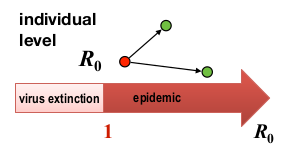
\includegraphics[width=0.9\textwidth]{../lessons/image/16/image02a.png}
\end{minipage}
\begin{minipage}[]{0.5\linewidth}
\centering
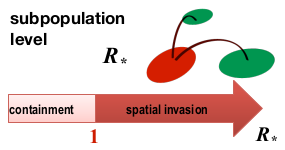
\includegraphics[width=0.9\textwidth]{../lessons/image/16/image02b.png}
\end{minipage}
\caption{\label{fig:16_02} \textbf{Left:} Dynamics of spread on a individuals-in-a-network level. \textbf{Right:} Dynamics of spreading among subpopulation, once we made a \textit{coarse graining}. Graphically, they look like similar, despite the change in value, and meaning, of parameters as output of the mapping. $R^*$ is the analogous of the basic reproductive ratio $R_0$ at metapopulation level.}
\end{figure}

We are indeed approximating as a \textbf{branching process} and try to follow the invasion dynamics at the subpopulation level, denoting by $D^n$ the diseased subpopulations at the $n$-th generation. Hence, we do not follow the dynamics in term of times, but in terms of \textit{generation}.


\subsection{Homogeneous networks}

Let us assume that we are dealing with \textbf{homogeneous systems}, for the sake of simplicity, and with only 2 patches: namely $j$ and $i$ as one can see in Fig. \ref{fig:16_03}.

\begin{figure}[h!]
\centering
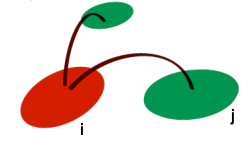
\includegraphics[width=0.34\textwidth]{../lessons/image/16/image03.png}
\caption{\label{fig:16_03} Dynamics of spatial spread at subpopulation level, but considering only two patches.}
\end{figure}

The variables one may want to introduce now are the following ones: $w_0$ is the \textbf{number of travellers} along each link, whereas $\expval{k}$ is on average the \textbf{number of connection} of each subpopulation, which coherently with our notation has \textbf{population} $N$. Let us introduce now $\alpha$, that is the \textbf{epidemic attack rate}: it is the \textit{"final size"} of the epidemic within each patch. We recall that the latter depends on the basic reproductive ratio $R_0$.

Using these quantities we can compute the probability of early extinction of the disease, that is the probability for the disease to be not able to spread to other patches once it started in patch $i$:
\begin{equation}
    P_{ext} = \qty( \frac{1}{R_0} )^{\lambda_{ij}}
\end{equation}
where $R_0$ is the usual term and $\lambda_{ij}$ is the total number of infectious individuals sent from $i$ to $j$ during the local outbreak:
\begin{equation}
    \lambda_{ij} = \frac{w_0}{\cancel{N}} \frac{\alpha \cancel{N}}{\mu}
\end{equation}
Note that the \textit{recovery rate} $\mu$ is included as well and the first ratio is the \textit{probability} to travel.

The number of diseased subpopulation at generation $n$, namely $D^n$, is computed iteratively from the number of diseased patches at generation $D^{n-1}$:
\begin{equation}
    D^n = (\expval{k}-1)(1-P_{ext}) \mathcolorbox{green!20}{\left( 1- \sum_{m=0}^{n-1} \frac{D^m}{V} \right) } D^{n-1}
    \label{eqn:D^n_first}
\end{equation}
where $V$ is the number of patches. Moreover, in the factor $(\expval{k} - 1)$, the $-1$ is present in order to ignore the patch we have got the infection from. In addition, the one highlighted is the probability that the patch is disease free at $n-1$-th generation. The last factor $D^{n-1}$ is the number of diseased patches at the previous generation: as one can imagine, if the remaining factor is \textbf{larger} than 1, then the epidemic has an outbreak, otherwise it gets extinct.

Accordingly to what we have just said, the factor $R_*$ is therefore defined \textit{at the beginning of the infection}, i.e. when all patches are susceptible and so the sum gives no contribution, as:
\begin{equation}
    R_* = (\expval{k}-1)(1-P_{ext})
\end{equation}
Moreover, if $R_0$ is really low\footnote{Actually this last approximation does not hold for $COVID19$, since it was able to spread given that its $R_0$ was high.}, the probability of having an outbreak is:
\begin{equation}
    1 - P_{ext} = 1 - \left(\frac{1}{R_0} \right) ^{\lambda_{ij}} \simeq \lambda_{ij} (R_0 - 1) = \frac{\alpha w_0}{\mu} (R_0 - 1)
\end{equation}
which actually simplifies our expression for $R_*$. Indeed, recalling that according to our assumption every patch has same number of connections and travellers, we obtain:
\begin{equation}
    R_* = (\expval{k}-1)\frac{\alpha w_0}{\mu} (R_0 - 1)
\end{equation}
We want now to study the \textbf{dependencies} of the \textbf{invasion potential}. It is indeed a \textit{growing} function of: $R_0$, both mobility related quantities \textit{overall traffic rescaling} $w_0$ and \textit{average number of connections} $\expval{k}$. In addition, it is \textit{inversely proportional} wrt recovery rate $\mu$ or, in other words, it is a \textit{growing} function of \textbf{infectious duration}. The more we stay infected the larger becomes $R_*$ and if the latter is larger than $R_* > 1$ the epidemic is able to spread to other patches, which actually makes sense.


\subsection{Heterogeneous networks}

Let us introduce a more realistic model and consider that networks are actually different from the homogeneous we have seen up to now. Indeed, \textbf{real systems} are \textbf{highly heterogeneous}. As we have already pointed out (see Sec. \ref{section:human_mobility} and Fig. \ref{fig:13_01} and \ref{fig:13_02}): the number of connections and travellers along the connections is heterogeneous\footnote{Colizza \& Vespignani, PRL 2007, JTB 2008}. This implies that average quantities, such as $\expval{k}$, are not representative of the properties of the patches: \textbf{homogeneous approximation is bad}.
However, we were able to find some \textbf{scaling relations}: that are some approximate laws that make computations feasible and describe the \textbf{degree-block} description (coarse-graining).

\begin{figure}[h!]
\centering
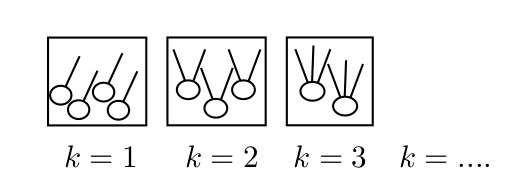
\includegraphics[width=0.45\textwidth]{../lessons/image/16/image04.png}
\caption{\label{fig:16_04} Patches are divided into different degree blocks, according to the number of connections $k$ they have.}
\end{figure}

With \textbf{degree-block} description we mean that we group patches according to their degree, and consider patches within the same degree-classes homogeneous. In other words, we make the approximation, similar to the one we have made with networks, that patches with \textbf{same number of connections behave in the same way}, like when we used the \textit{Mean Field Degree Approximation} with networks.

We can rewrite some quantities using some empirical laws found when analyzing air traveling data: catchment populations, number of connections for every airport etc. The number of individuals resident in the patch $k$ is:
\begin{equation*}
    N_k = N_0 k^\phi
\end{equation*}
Whereas the flux between two nodes $k$ and $k'$:
\begin{equation*}
    w_{kk'} = w_0 (k k')^\theta
\end{equation*}
therefore the \textbf{probability} of \textbf{travelling} from a node of degree $k$ to a node of degree $k'$ is:
\begin{equation}
    p_{kk'} = \frac{w_0}{N_0}\frac{(k k')^\theta}{k^\phi}
\end{equation}
where the $\phi, \theta$ are empirical values. Once we have as \textbf{input} the \textbf{degree distribution} $P(k)$, we can try to find the number of diseased subpopulations at generation $n$, with $k$ mobility connections, namely $D_k^n$.

\begin{figure}[h!]
\centering
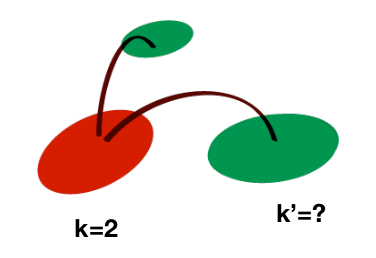
\includegraphics[width=0.34\textwidth]{../lessons/image/16/image05.png}
\caption{\label{fig:16_05} A patch that has $k=2$ connections was infected. We want to compute what is the probability that it is connected to a disease-free patch of degree $k'$.}
\end{figure}

We want now to derive the invasion equation as before, but this time in a heterogeneous mean field approach framework. The question to be replied is therefore the following: \textit{what is the probability that an infected patch with degree $k$ is connected to a disease-free patch of degree} $k'$. The answer to this question is the following:
\begin{equation}
    D_k^n = \sum_{k'}D_{k'}^{n-1} \mathcolorbox{green!20}{(k'-1) P (k'|k)} \mathcolorbox{red!20}{\qty( 1-\sum_{m=0}^{n-1} \frac{D_{k'}^m}{V_{k'}} ) } \mathcolorbox{orange!20}{ (1-P_{ext}(\lambda_{k'k})) }
    \label{eqn:D_k^n}
\end{equation}
which looks like \ref{eqn:D^n_first}, except for the sum over all possible degrees $k'$ that was introduced since we are dividing our patches in same-degree classes. Let us analyze every term: the $k-1$ is the number of mobility connections through which the seeding may potentially occur. This is multiplied by the probability that contact has degree $k'$, given we are starting from a node with degree $k$: explicitly \textit{in random networks} $P(k'|k) = k' \frac{P(k')}{\expval{k}}$. In this step, we have assumed that the network is uncorrelated. This however implies that when we are making connections at random we are more likely to connect to hubs, leading to the so called \textit{friendship paradox}, a.k.a. "rich gets richer", where nodes that have already many connections tend to accumulate more. These last two terms are given by the \textbf{topology} of the network.
The second last term (red) is equal to the one previously obtained: it is indeed the probability that the contact patch belonging to $k'$ class is disease-free. Last term (orange) is, as before, the probability for the epidemic to not get extinct before the global outbreak.
One should note that, as previously done, this last term can be approximated to $\lambda_{k' k}(R_0 - 1 )$ assuming this is a \textit{branching process}, and moreover for heterogeneous networks:
\begin{equation*}
    \lambda_{k' k} = \frac{w_0 (k k')^\theta}{ \cancel{ N_0 k^\phi}} \frac{\alpha}{\mu} \cancel{ (N_0 k^\phi) }
    = w_0 (kk')^\theta \frac{\alpha}{\mu}
\end{equation*}
Finally, \ref{eqn:D_k^n} can be rewritten as it follows:
\begin{equation}
     D_k^n = (R_0 - 1)
     \frac{\alpha w_0}{\mu}
     \frac{k^{1+\theta}P(k)}{\expval{k}} \sum_{k'}
      \mathcolorbox{red!20}{D_{k'}^{n-1} (k'-1) k'^{\theta }}
    \label{eqn:D_k^n_second}
\end{equation}
If we define the highlighted factor in red as $\Theta^{n-1}$ for a more compact writing, we can multiply both rhs and lhs of Eq. \ref{eqn:D_k^n_second} by $\sum_k (k-1)k^\theta$ thus obtaining:
\begin{equation}
    \Theta^n = (R_0 - 1) \frac{\alpha w_0}{\mu} \frac{\expval{k^{2+2\theta}}- \expval{k^{1+2\theta}}}{\expval{k}} \Theta^{n-1}
\end{equation}
In this way we obtain a function that is monotone as well and has the property that the epidemic spreads if $\Theta^n$ is greater than $\Theta^{n-1}$. But, actually, this how $R_*$ works, so we have found an expression for the \textbf{invasion potential}:
\begin{equation}
    R_* = (R_0 - 1) \frac{\alpha w_0}{\mu} \frac{\expval{k^{2+2\theta}}- \expval{k^{1+2\theta}}}{\expval{k}} > 1
    \label{eqn:R_*_def}
\end{equation}
If the last condition holds, then the epidemic will spread. As one can easily note, $R_*$ is a growing function of $R_0$, the overall traffic rescaling and average number of connections ($w_0$), epidemic attack rate $\alpha$, infectious duration ($\tau = \mu^{-1}$) and, finally, of the \textbf{moments of the degree distribution and its fluctuations} which are very large for random networks: $\expval{k^{2+2\theta}}- \expval{k^{1+2\theta}} \approx 7\cdot 10^4$ while $\expval{k}= 10$. In this way, the network topology is indeed \textit{helping} and \textit{favoring}
 the spread of the disease (see Fig. \ref{fig:16_06})!
One should keep in mind that we are dealing with travelling individuals as integers, and the stochasticity relies in the process of travelling, which might either happen or not (Bernoulli process). However, if they are treated as integers we are not sure that outbreak will happen for sure. Indeed, this would happen when dealing with continuous variables (i.e. fraction of individual) which would be quite unrealistic.

\begin{figure}[h!]
\begin{minipage}[c]{0.5\linewidth}
\centering
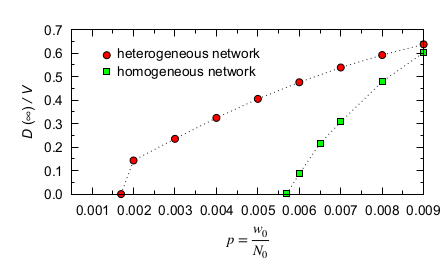
\includegraphics[width=0.9\textwidth]{../lessons/image/16/image06a.png}
\end{minipage}
\begin{minipage}[]{0.5\linewidth}
\centering
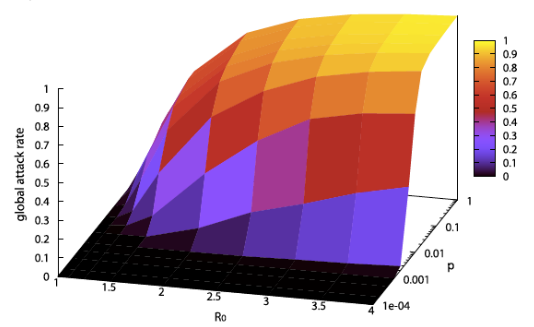
\includegraphics[width=0.9\textwidth]{../lessons/image/16/image06b.png}
\end{minipage}
\caption{\label{fig:16_06} \textbf{Left:} Network topology favors the spreading of the disease and its global outbreak. \textbf{Right:} Attack rate in function of different traveling probabilities and the basic reproductive ratio $R_0$.}
\end{figure}

\section{Spatial spread of competing diseases}

\begin{figure}[h!]
\centering
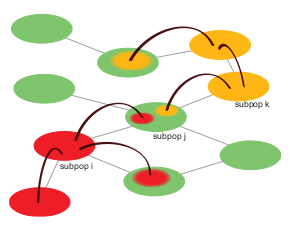
\includegraphics[width=0.34\textwidth]{../lessons/image/16/image07.png}
\caption{\label{fig:16_07} Two strains present in the same metapopulation network.}
\end{figure}

We will present now an application to understand better what we have explained so far: let us assume that there are two \textbf{competing pathogens} that are in the same metapopulation system. The \textbf{compartmental} model\footnote{Poletto, PLOS Comp Biol PRL 2007, JTB 2008.} that we obtain is the one in figure \ref{fig:16_08}: there are two strains of a certain disease present, and one individual might be infected by either one of them. Once he recovers, he acquires the \textbf{full-cross immunity}, that is to say that he cannot be infected by both of them any more. The main difference between the two is that the infectious period of one is actually \textbf{faster} than the others ($\tau_{slow} > \tau_{fast}$), whereas they share the \textbf{same} $R_0$.

\begin{figure}[h!]
\centering
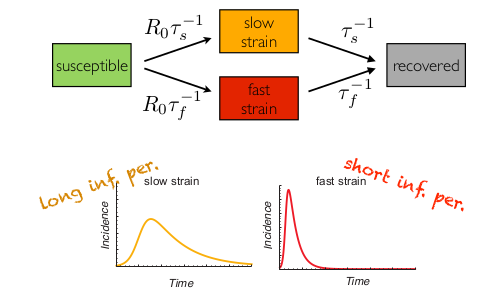
\includegraphics[width=0.7\textwidth]{../lessons/image/16/image08.png}
\caption{\label{fig:16_08}\\
\textbf{Top.} Compartmental model for two competing disease with same $R_0$ and different infectious time $\tau$. Once one recovers, he acquires the full cross immunity.
\textbf{Bottom.} Different epidemic timescales for the fast and slow strain of the disease.}
\end{figure}

Since the two strains have actually different infectious periods, they lead to \textbf{different infectious dynamics}. Indeed, $\tau$ affects both the slope of the \textit{exponential growth}, as well as the \textit{peak} and the presence of the disease at longer times. For instance, keeping $R_0 \propto \beta/\mu $ \textbf{fixed}, if $\tau$ is small we stay infected for less time but the transmissibility $\beta$ must be actually higher, hence the spreading explodes. On the other hand, if $\tau$ is large, we stay infected more and therefore the disease has more time to spread despite the lower $\beta$. At the end of the epidemic, we will have reached the same amount of population but ended up with very different dynamics.

If we let the two different disease spread in a \textbf{well-mixed population} with the same assumptions as before: the faster strain will infect faster much more people, being the transmissibility higher. In a certain sense, the "slow" disease will \textit{die out}.

Let us now \textbf{introduce}, under the same assumptions of two competing diseases one faster than the others with fixed $R_0$, the \textbf{metapopulation network}. The probability to travel from a patch to another is $p$, regardless of the patches. The results of the simulation are depicted in figure \ref{fig:16_09}.

\begin{figure}[h!]
\centering
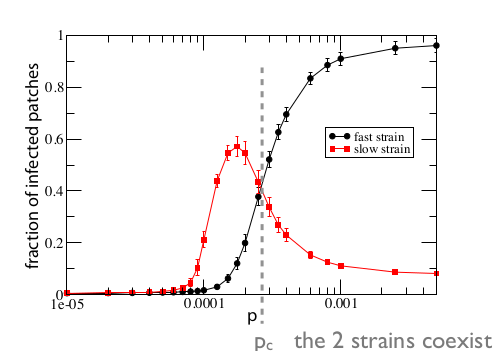
\includegraphics[width=0.6\textwidth]{../lessons/image/16/image09.png}
\caption{\label{fig:16_09} Numerical simulation results for two competing strains in metapopulation networks for different value of travelling probability.}
\end{figure}

At the end of simulation there might be a little chance for the two strains to coexist if they reach the same patch, however, more likely the fast strain will make the other die out when the \textit{probability of travelling} is \textit{higher}. On the other hand, if the \textit{travelling probability} is \textit{less} they even might not encounter each other, and therefore the slower strain is favored to last longer and still be present at the end of simulation time. We can find a \textbf{probability} $p_c$ for which the two diseases coexist. One should note that, for higher traveling probability, we approach the \textit{homogeneous mixing regime}.

Recalling what we have discussed, we can bring what is at the scale of individuals, namely the infection duration $\mu^{-1}$, $R_0$ and the logistic curve $I(t) \sim e^{\mu(R_0-1)t}$ to a \textbf{patches scale}. The timescale will be the \textit{outbreak duration} $T$ and $R_*$ will be:
\begin{equation}
R_* = (\expval{k}-1) \frac{\alpha p N}{\mu} (R_0 - 1)
\end{equation}
while the \textbf{number of diseased} patches is $D(t) \sim e^{\frac{1}{T}(R_* - 1) t}$. One should note that, since we are assuming that all patches are the same, the outbreak duration $T$ on average is the same for every patch.

According to the fact that $R_*$ is an increasing function of $\mu^{-1}$, we have that the invasion potential $R_*^s > R_*^f$. However, for \textit{large} $p$ it holds that both $R_*^s, R_*^f \gg 1$, but the faster strain is able to reach more rapidly new patches.
Instead, for \textit{small} $p$, we have $R_*^s > R_*^f$ and the slower strain is more able to percolate through the system.

We want now to understand how the probability $p_c$ for the \textbf{crossover} changes with respect of $R_0$. We need to solve the following equation:
\begin{equation}
    \frac{D_s(t)}{D_f(t)} \sim e^{\left( \frac{R_*^s -1}{T_s}- \frac{R_*^f -1}{T_f}\right) } = 1
\end{equation}
The solution is plotted in the left image of Fig. \ref{fig:16_10}.
It is given by replacing the value for $R_*$, keeping also in mind that in homogeneous mixing $T_s = T_f$.  In this way, it becomes reasonable to be solved, otherwise a graphical approach would have been needed.

\begin{figure}[h!]
\begin{minipage}[c]{0.5\linewidth}
\centering
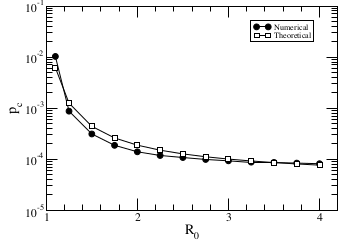
\includegraphics[width=0.9\textwidth]{../lessons/image/16/image10a.png}
\end{minipage}
\begin{minipage}[]{0.5\linewidth}
\centering
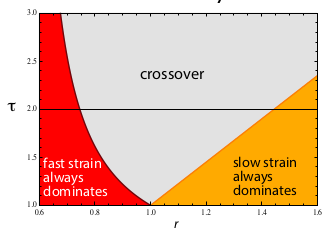
\includegraphics[width=0.9\textwidth]{../lessons/image/16/image10b.png}
\end{minipage}
\caption{\label{fig:16_10} \textbf{Left:} Crossover probability for different Basic reproductive rate $R_0$. \textbf{Right:}\\ Two competing strains in homogeneous metapopulations with different $\tau$ and different $R_0$.}
\end{figure}

Now let us \textbf{drop} the assumption that $R_0$ is \textbf{fixed}, and allow for different $R_0$\footnote{Poletto et al. Sci Rep 2015.}:
\begin{equation}
    R_0 ^ s = r R_0^f
\end{equation}
where $r$ is the ratio between the two $R_0$ and $\tau$ (see Fig. \ref{fig:16_10}) is the ratio between the two infectious periods.
Now, things start to change, indeed there are some regions where \textbf{regardless} of the level of \textbf{mobility} either one of the two strain dominates: this happens quite always for limiting cases wrt $r$. For \textit{small} $r$ fast strain \textit{always} dominates regardless the time of infection, while for \textit{large} $r$ slow strain always dominates when $\tau$ is not so large. There is in addition a \textbf{crossover} region where the two may coexist and \textbf{mobility} does \textbf{not} matter.

Analytically, if we introduce the exponential growth in homogeneous mixing as $G=\mu(R_0 -1)$, we see that:
\begin{equation}
    G^s > G^f \implies R_*^s > R_*^f, \qquad R_*^f > R_*^s \implies G^f > G^s
\end{equation}
that defines our colored areas where either one strain dominates (the one that comes with larger $R_*$). However, if $G^f > G^s$ \textit{and} $R_*^s > R_*^f$ we may observe \textbf{crossover}.
More particularly:
\begin{subequations}
\begin{align*}
  r>1 \rightarrow \quad & G^f > G^s \quad \Rightarrow \quad r R_0^f - 1 < \tau \qty(R_0^f-1) \\
  r<1 \rightarrow \quad & R_*^s > R_*^f \quad \Rightarrow  \quad  \tau  \alpha _s \log (R_0^s) > \alpha _f \log (R_0^f)
\end{align*}
\end{subequations}




\end{document}
